\documentclass[11pt]{article}

\usepackage{amsmath}
\usepackage{amsfonts}
\usepackage{amssymb}
\usepackage{amsthm}
\usepackage{graphicx}
\usepackage{graphicx}
\usepackage{tikz}
\usepackage{pgfplots}
\usepackage{setspace}
\usepackage{fullpage}
\usepackage{color}
\usepackage{xcolor,colortbl}
\usepackage{comment}
\usepackage{bm}
\usepackage{url}
\usepackage{hyperref}
\usepackage{color,hyperref}
\definecolor{darkblue}{rgb}{0.0,0.0,0.3}
\hypersetup{colorlinks,breaklinks,
            linkcolor=darkblue,urlcolor=darkblue,
            anchorcolor=darkblue,citecolor=darkblue}

%Change to Helvetica
%\usepackage[scaled]{helvet}
%\renewcommand*\familydefault{\sfdefault} %% Only if the base font of the document is to be sans serif
%\usepackage[T1]{fontenc}

%Change to fourier
%\usepackage{fourier}
%\usepackage[T1]{fontenc} 

\usepackage[T1]{fontenc}
\usepackage{charter}
\usepackage[expert]{mathdesign}

\begin{document}
\noindent \textbf{Problem Set 1 - PS 402 DUE Friday 9/30 6pm \color{gray} ANSWER KEY}

\begin{enumerate}
\item Exponents and Logarithms
\begin{enumerate}
\item Multiply $x^4 y^3 z^2 (1 + x^2 y^2)$ \color{gray} $x^4y^3z^2+x^6y^5z^2$\color{black}
\item Simplify $((xy)^{-6})^{0.5} y^3z^{3}$ \color{gray} $\frac{z^3}{x^3}$ or $(\frac{z}{x})^3$\color{black}
\item Simplify $((xy)^2)^{1.5} x^{-3}y^{-3}$ \color{gray} $1$\color{black}
\item Solve for $ln(e^5/e^{2.5})$ \color{gray}$2.5$\color{black}
\item Simplify $e^{ln 7.14}$ \color{gray} $7.14$\color{black}
\item What is $log_{7134\pi}(1)$? \color{gray}$0$ (log 1, with any base, is always zero)\color{black}
\item Solve for x $log_x(16)=4$ \color{gray}2 \color{black}
\item Combine into one term: $log(3x)+2log(y)$ \color{gray}$log(3x*y^2)$ \color{black}
\end{enumerate}

\item Inequalities and Absolute Values
\begin{enumerate}
\item ``Solve'' for $x$: $x + y +2 < 4$  \color{gray} $x < 2-y$\color{black}
\item ``Solve'' for $x$: $(-4)(x + 7) \geq -24$ \color{gray} $x \leq -1$\color{black}
\item What is the absolute value of $-24$? \color{gray} $24$\color{black}
\item Graph $y = |x +2|$ \color{gray} \color{black}


\begin{tikzpicture}
        \begin{axis}[%
            domain = -3:1,
            samples = 100,
            axis x line = center,
            axis y line = center,
            xlabel = {$x$},
            ylabel = {$y$},
            ticks = none
            ]
            
            \addplot[gray] {abs(x+2)} [yshift=3pt] node[pos=0.41,left] {$y=|x+2|$};
        \end{axis} 

\end{tikzpicture}
\vspace{2mm}

\item On number line, graph $|x + 2| \geq 3$ \color{gray} $x \geq 1, x \leq -5$\color{black} \\

	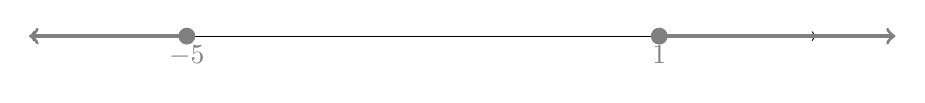
\begin{tikzpicture}
	\vspace{2mm}
		\draw[<->] (-7, 0) -- (3, 0);
		\draw[fill=gray, gray] (-5, 0) circle (1mm) node[below] {$-5$};		
		\draw[fill=gray, gray] (1, 0) circle (1mm) node[below] {$1$};	
		\draw[->, very thick, gray] (1, 0) -- (4, 0);
		\draw[->, very thick, gray] (-5, 0) |- (-7, 0);
	\end{tikzpicture}
\item On number line, graph $|x - 7| < 1$ \color{gray} $6 < x < 8$\color{black} \\

	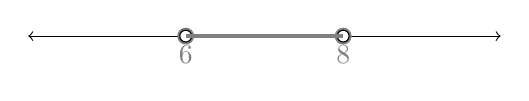
\begin{tikzpicture}
	\vspace{2mm}
		\draw[<->] (4, 0) -- (10, 0);
		\draw[fill=gray, gray] (6, 0) circle (1mm) node[below] {$6$};
		\draw[fill=white] (6, 0) circle (0.75mm) ;		
		\draw[fill=gray, gray] (8, 0) circle (1mm) node[below] {$8$};	
		\draw[fill=white] (8, 0) circle (0.75mm) ;
		\draw[ very thick, gray] (6, 0) -- (8, 0);
	\end{tikzpicture}
	
\item On number line, graph $|2x - 2| = 4$ \color{gray} $x=-1, 3$\color{black} \\

	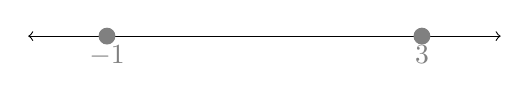
\begin{tikzpicture}
	\vspace{2mm}
		\draw[<->, black] (-2, 0) -- (4, 0);
		\draw[fill=gray, gray] (-1, 0) circle (1mm) node[below] {$-1$};		
		\draw[fill=gray, gray] (3, 0) circle (1mm) node[below] {$3$};	

	\end{tikzpicture}
\end{enumerate}

\item Factor
\begin{enumerate}
\item $x^2+ 5x+4$ \color{gray} $(x+1)(x+4)$\color{black}
\item $6m^2+8m-8$  \color{gray} $(3m-2)(2m+4)$ \emph{or} $2(3m-2)(m+2)$\color{black}
\item $5y^2-12yz+7z^2$ \color{gray} $(5y-7z)(y-z)$\color{black}
\end{enumerate}

\item Functions
\begin{enumerate}
\item What is the difference between a function and relation (in words)? \color{gray} A function cannot map two elements from the domain to the range.  \color{black}

\item Simplify $h(x)=g(f(x))$, where $f(x)=x^2+4$ and $g(x)=\sqrt{x-4}$ \color{gray}f(g(x))=x \color{black}

\item Find the inverse function of $f(x)=5x-3$ \color{gray}The inverse is: $(3+x)/5$ \color{black}
%. 
\item What is a quadratic function? (define and provide example) \color{gray}Highest degree of 2--example $y=x^2+x+a$ \color{black}
\item Why do we care if a function is monotonically doing anything? \color{gray} We are often specifying a relationship between variables and our outcome -- we want to know, is more of x ALWAYS associated with more (or less) of y? Sometimes? Is there a peak? This language can help explain the relationship. \color{black}
\end{enumerate}


\item Exponent(ials)
\begin{enumerate}
\item Explain the difference between, and provide an example of, the following. Be sure to use an example different from the slides: 
	\begin{enumerate}
	\item Exponent: \color{gray} A number multiplied by itself a set number of times (variable to a power, e.g. $x^2$) \color{black}
	\item Exponential: \color{gray} A number multiplied by itself some unknown number of times (number to a variable, e.g. $3^x$) \color{black}
	\item Exponential Function:  \color{gray} A particular number ($e$) to an unknown power (e.g. $e^3x$) \color{black}
	\end{enumerate}
\end{enumerate}


\item Identification
\begin{enumerate}
\item Identify the following greek letters by name. Include the meaning and common usage if you are able. 
\begin{enumerate}
\item $\delta$ \color{gray}  delta: derivatives \color{black}
\item $\beta$ \color{gray}  beta: coefficient \color{black}
\item $\alpha$ \color{gray}  alpha: often a constant \color{black}
\item $\theta$\color{gray}  theta: often a variable \color{black}
\item $\lambda$ \color{gray} lambda: often for matrix (linear) algebra \color{black}
\item $\mu$\color{gray}  mu: means \color{black}
\item $\Delta$ \color{gray}  Delta (uppercase): change \color{black}
\end{enumerate}

\item Identify the following mathematical symbols by name. Include the meaning/usage. 
\begin{enumerate}
\item $\in$ \color{gray} In (set theory) \color{black}
\item $\cup$ \color{gray} Union (set theory) \color{black}
\item $\subset$ \color{gray} Subset (set theory) \color{black}
\item $\wedge$ \color{gray} And (logic) \color{black}
\end{enumerate}
\end{enumerate}

\item Necessary and Sufficient \color{gray} Examples vary \color{black}
\begin{enumerate}
\item Provide an example of a necessary condition \color{gray} A necessary condition is one where we observe the outcome if an only if we observe the condition.  \color{black}
\item What is the difference between necessary and sufficient? \color{gray} A sufficient condition must be present for the outcome to occur, but its presence does not guarantee the outcome. That is, if temperature is a sufficient condition, it needs to be hot for it to rain, but if it's hot, it may or may not rain. \color{black}
\end{enumerate}
\end{enumerate}


\begin{comment}
\item Summation
\begin{enumerate}
\item $\sum_{n=1}^{7}3$ \color{gray} $7*3=21$\color{black}
\item $\sum_{n=0}^{4} 2n+8$ \color{gray} $\sum_0^4 2n+ \sum_0^4 8= \frac{2*4(5)}{2}+5*8=60$  \color{black}
\end{enumerate}

\item Set theory
\begin{enumerate}
\item In roster notation, write the set characterized in set-builder notation as $S = \{x \in \mathbb{Z}, 2 <x <5\}$. \color{gray} $\{ 3,4\}$\color{black}
\item Graph on the number line the interval $[-3, 2)$. \color{gray} Need open circle\color{black}
\item Is the following statement True or False? $\forall x \in S, x\geq 2$ for $S = \{3,2,5,9\}$. \color{gray} T. All values are greater than or equal to 2. \color{black}
\item Is the following statement True or False? $\exists x \in S\; s.t. \; x \notin \mathbb{Z}$ for $S = \{3,2,5,9\}$. \color{gray} F. All numbers in the set are integers and thus no element is not a member of the set of integers. \color{black}
\item Is $\{1,2,3,4\}$ a subset of $\{4,3,1,2\}$? Is it a proper subset? \color{gray} It is a subset, but not proper subset because there are no elements in the second that are not elements of the first set. \color{black}
\item Using logical symbols (including $\exists$ and $\forall$) write the definition of a proper subset.  \color{gray} Took most answers as long as they looked `mathy'. Wanted some version of $A \subset B \leftrightarrow  x \in A \rightarrow x\in B \wedge \exists y\in B | y \notin A $ \color{black}
\item If $A = \{\text{soup}, 8\}$ and $B = \{x, \text{soup}\}$ find $A \cup B$. \color{gray} $A \cup B= \{ \text{sou}. 8, x \}$\color{black}
\item (Follow-up): Now find $A \cap B$. \color{gray} $A \cap B= \{ \text soup\}$\color{black}
\item (Follow-up): Find the Cartesian Product $A \times B$. $A \times B = \{ (\text{soup}, x), (\text{soup}, \text{soup)}, (8, x), (8, \text{soup})\}$ \color{black}
\end{enumerate}




\item Introduction to differentiation
\begin{enumerate}
\item What is a derivative? Why might we find it useful? \color{gray} A derivative enables us to do many different things, primarily understand rates of change at particular points and patterns of change overall. It also enables us to find maxima and minima. \color{black}

\item Give an example of a derivative we might care about (think about the education and salary graphs from lecture) \color{gray} Many examples work: Arrival/exit in the workforce and national GDP, disease rates, vaccination rates, just about anything that you can look at over time. \color{black}

\item If $f(x) = x^2$ and $g(x)= 3x + 9$, write $z(x) = f(g(x))$ and simplify (i.e. expand). \color{gray} $z(x)=(3x+9)^2=9x^2+54x+81$ \color{black}

\item Compute manually, using the formula for a derivative (i.e. $ lim_{h\rightarrow0}\frac{f(x+h)-f(x)}{h}$), the derivative of $x^3$. \color{gray} $lim_{h\rightarrow0}\frac{(x+h)^3-x^3}{h}=lim_{h\rightarrow0}\frac{x^3+3x^2h+3xh^2+h^3-x^3}{h}=lim_{h\rightarrow0}\frac{3x^2h+3xh^2+h^3}{h}=lim_{h\rightarrow0}3x^2+3xh+h^2=3x^2$ \color{black}


\item Find the derivative of $f(x) = 2x^2 + 7x + 9$. \color{gray} $f'(x)=4x+7$ \color{black}

\item Find the derivative of $f(x) = 3x^2$ \color{gray} $f'(x)=6x$ \color{black}
\end{enumerate}
\end{enumerate}


\end{comment}


\end{document}




